
\section{Supporting Flyspeck in a Semantic Wiki}

Starting from a minimal set of requirements, we have evaluated the
applicability of two concrete semantic wikis to Flyspeck.  We used two
different frameworks: a prototype developed on top of Semantic
MediaWiki, and our own semantic wiki SWiM. 

\subsection{Motivation}
\label{sec:req}

The Flyspeck project has garnered significant enthusiasm in the theorem proving
community: Hales has given talks about the project at a number of prestigious
conferences, and aspects of Flyspeck are currently a motivation behind 
one complete and at least
two current PhD dissertations.  At present, however, Flyspeck is not ready for
crowdsourcing.  Because definitions rely so heavily on each other, and the lemma
statements rely on the definitions, Hales needs to oversee the computerization
of the definitions so that the mathematical constants are correct\footnote{For
  example, one can represent a vector as a function from the integers to the
  reals, or as a tuple of reals.  The operations of vector spaces will depend on
  this representation, etc.}.  Once the formal definitions are complete, the
rest of the project can proceed practically in parallel by
many independent collaborators.

To build a prototype, we computerized the definitions and lemma statements of
the first chapter of the book (Trigonometry) in the
Twelf\cite{Schurmann:1999:Twelf} proof assistant.  Then we
listed a minimal set of behaviors the wiki should support.

\subsection{Requirements}

Our focus in this work is on making the extent and structure of
Flyspeck comprehensible and on communicating where work needs to be
done.  For this the outline of the whole proof from the
book\cite{Hales:2007:FlyspeckBook} needs to be represented in the
wiki, where the mathematical statements (including definitions,
lemmas, and theorems) are available in a human-readable way (with
formulae in \LaTeX\ or presentational MathML) as well as a
computerized presentation suitable for downloading into a theorem
prover.  In order to obtain a well-structured network of knowledge
items, each mathematical statement should be presented on one wiki
page, which shows its human-readable representation from the book,
offers additional space for annotation, and allows for downloading a
formal representation.  

An example usage scenario is as follows. A user wishes to contribute to
Flyspeck.  She looks at our wiki main page, which shows her what still needs to
be done.  Preferring analysis to geometry, she searches for open problems
involving analysis.  This returns a list of lemmas related to analysis from
which she can choose one that seems possible given her time constraints. She
downloads the relevant formal definitions and lemmas, along with the text of a
paper proof culled from Hales' book.  She uses a proof assistant to begin
formalizing the paper proof.  At some point, she needs
clarification on some definition and additionally has an idea on how to
generalize this lemma.  She thus asks for help and makes comments in a forum
space of the wiki.  She completes her proof, and uploads the proof assistant
file to the wiki.  The wiki uses a theorem prover to check the proof for
correctness and, if it is correct, adds it to the database.

With this scenario in mind, we propose that the wiki should minimally offer: 
\begin{description}
\item[A knowledge base] of the theory, constant, and lemma definitions.
\item[A theory browser] where a user can browse the knowledge by category, or search with keywords.
\item[A download area] where one can download the definitions, lemmas, and existing proofs.
\item[An upload area] where one can upload new proofs.
\item[A forum] to discuss issues involved in the formalizations.
\end{description}

The following set of annotations should support this minimal infrastructure:

\begin{description}
\item[Categorization by topic:] In the beginning, one would mirror the narrative structure
  of the book (e.\,g.\ ``sphere'' being a subsection of ``primitive volumes'', which in turn
  is a section of the chapter ``volume calculations'').  Standardized ways of classifying
  mathematical topics, such as the Mathematical Subject Classification
  (MSC)\cite{AMS:MSC2000}, could be added later.
\item[Project-organization metadata] such as whether the proof
  of a lemma has already been computerized, or if someone is currently 
  attempting a proof.  This is essential so that two people don't duplicate
  work.
\item[Dependency links:] These can be links from individual symbols in
  mathematical formulae to the place where they are declared, or from
  any page $p$ to other pages containing knowledge that is required
  for understanding $p$: either pages in the same wiki, or external
  resources like \product{PlanetMath} or \product{Wikipedia} articles.
\item[Discussion posts] should be strongly tied to the topic being
  discussed, and classified into categories like question, answer,
  explanation, etc.
\end{description}

There should be an enticing page for visitors and potential
collaborators that gives an impression of the extent and structure of
the project (e.g. its size and its specialization into diverse fields
of mathematics).  For the developer, there should be tools for
browsing and querying the knowledge.  Not only should it be possible
to query knowledge items by their annotations, but important query
results must also be available as dynamically generated lists.
Examples for queries are:

\begin{enumerate}
\item\label{item:proven-lemma} ``Which lemmas about composite regions need
  to be proved?''
\item ``What lemmas are difficult to prove?''
  \begin{enumerate}
  \item \ldots in the sense that many people have already attempted them, but given up
  \item\label{item:question-count} \ldots in the sense that many people have asked
    questions in the related discussion
  \end{enumerate}
\item ``Are there textual resources I can read in order to understand the Jordan
  Curve Theorem?''
\item ``What other lemmas could help me to prove this one?'' (e.\,g.\ because
  they prove a related statement)
\end{enumerate}

A volunteer who is willing to work out and contribute a computerized proof for
a lemma should be able to download a self-contained computerized
representation of this lemma and everything it depends on.  Different
notions of ``dependency'' can be supported,
the most straightforward being that a lemma depends on the
declarations and definitions of all symbols it uses and on the transitive
closure of all symbols used by the latter.  Related lemmas
could be downloaded and assumed as axioms, under the assumption that
those will be proved later, perhaps by other collaborators.  
Assuming that the Flyspeck book is written in a
linear order, all definitions and lemmas \emph{before} the current one in the
narrative order could be used.

\newcommand{\wikipage}[5]{\node[draw,text width=5cm,font=\tiny\sffamily] (#1) at #2 {
    {\footnotesize\bfseries #3}\\
    #4
    ~\\[1em]
    [Download Twelf representation]\\
    #5
  };}
\begin{figure}
  \centering
  %\vspace{-.5cm}
  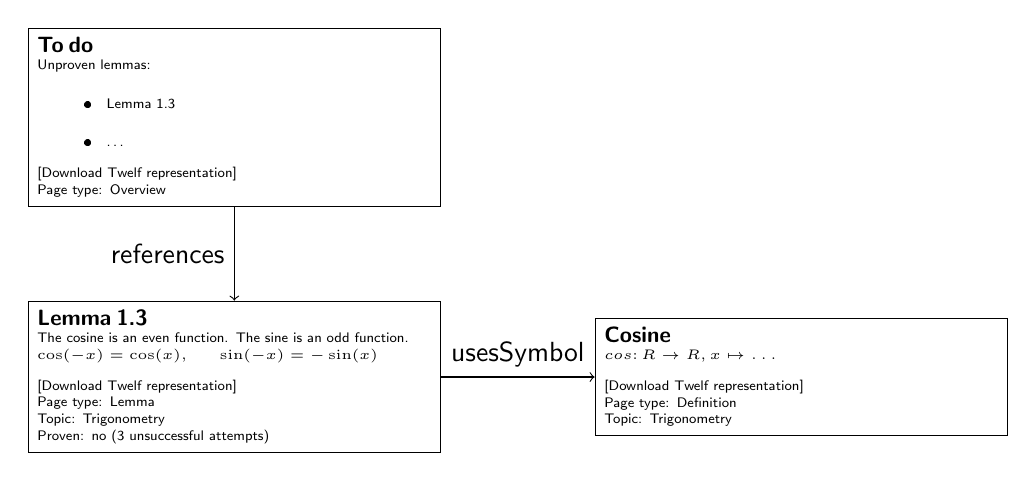
\begin{tikzpicture}[set style={{default}+=[scale=1.5,font=\sffamily]},default,xscale=.8]
    \wikipage{lemma}{(0,0)}{Lemma 1.3}{The cosine is an even function.  The sine is an odd function.\\
      $\cos(-x)=\cos(x),\qquad\sin(-x)=-\sin(x)$}{Page type: Lemma\\
      Topic: Trigonometry\\
      Proven: no (3 unsuccessful attempts)}
    \wikipage{cos}{(6,0)}{Cosine}{$cos\colon\mathbb{R}\to\mathbb{R},x\mapsto\ldots$}{
      Page type: Definition\\
      Topic: Trigonometry
    }
    \wikipage{todo}{(0,2.2)}{To do}{Unproven lemmas:
      \begin{itemize}
      \item Lemma 1.3
      \item \ldots
      \end{itemize}\vspace{-.5cm}
    }{
      Page type: Overview
    }
    \draw[->] (lemma) -- node[above] {usesSymbol} (cos);
    \draw[->] (todo) -- node[left] {references} (lemma);
  \end{tikzpicture}
  \caption{Page structure}
  \label{fig:pagestructure}
\end{figure}

During the formalization of the knowledge, we anticipate that the definitions
will undergo refactoring in order to facilitate the actual development of the
proofs.  (Historically, this has been the case with many large computerized
proofs, cf. \cite{Gonthier:2005:FourColor}.)  Refactoring support by the wiki
would thus be advantageous.

%%% Local Variables: 
%%% mode: latex
%%% TeX-master: "flyspeck-wiki-eswc08"
%%% End: 
